\documentclass{exam}

\usepackage[top=0.9in, bottom=1in, left=1.5in, right=1.5in]{geometry}
\usepackage[utf8]{inputenc}
\usepackage[icelandic]{babel}
\usepackage[T1]{fontenc}
\usepackage[sc]{mathpazo}

\usepackage[parfill]{parskip}
\usepackage{booktabs,tabularx}
\usepackage{multirow}
\usepackage{enumerate}
\usepackage{graphicx}
\usepackage{amsmath, amsfonts, amssymb, amsthm}
\usepackage{tikz}
\makeatletter % Fix due to (recent versions of?) minted containing their own framed definition
\expandafter\providecommand\expandafter*\csname ver@framed.sty\endcsname
{2003/07/21 v0.8a Simulated by exam}
\makeatother
\usepackage{minted} %Minted and configuration

\usepackage[pdftex,bookmarks=true,colorlinks=true,pdfauthor={Eirikur Ernir Thorsteinsson},linkcolor=blue,urlcolor=blue]{hyperref}

\setcounter{secnumdepth}{-1} 
\hyphenpenalty=5000


% Picture locations
\graphicspath{{./Pics/}}

\usemintedstyle{default}
\renewcommand{\theFancyVerbLine}{\sffamily \arabic{FancyVerbLine}}

\newcommand{\Mod}[1]{\ \text{mod}\ #1}

\runningfooter{\hspace{-2cm}
\includegraphics[width=0.5\textwidth]{Pics/hi-von-logo}}{}{}

\renewcommand{\solutiontitle}{\noindent\textbf{Mögulegt svar:}}

\author{}
\date{}

\footer{}{}{}


\title{Stærðfræðimynstur í tölvunarfræði \\ Skilaverkefni 10}
\author{}

\printanswers

\begin{document}
\maketitle
\thispagestyle{empty} 

Skila skal þessu verkefni á vefnum \href{https://gradescope.com/}{Gradescope}. Aðgangskóði fyrir námskeiðið er \textbf{926WD9}.


\section{Spurningar}

\begin{questions}

\section{Kafli 10.4}

\question Útskýrið af hverju þessi net hafa engar brýr.

\begin{enumerate}[a)]
 \item $C_n$ með $n \geq 3$
 \item $K_{m,n}$ með $m \geq 2, n \geq 2$
\end{enumerate}

\paragraph{Í bók:} Hluti af Exercise 10.4.48

\question Gömul þraut snýst um raunir bónda nokkurs við að ferja úlf, geit og kálpoka yfir á. Bóndinn á einungis lítinn bát, svo hann getur einungis flutt einn hlut eða eina skepnu yfir í einu, auk sjálfs sín. Bóndinn getur ferjað hlutina fram og til baka að vild, en ekki er hægt að skilja geitina eina eftir með kálpokanum (því þá étur geitin kálið) og ekki er hægt að skilja úlfinn eftir eftirlitslausan með geitinni (því þá étur úlfurinn geitina).

Lýsum mögulegu ástandi í þrautinni með röðuðu pari. Til dæmis, þá er $(BG,UK)$ það ástand þar sem bóndinn og geitin eru á fyrri bakkanum en úlfurinn og kálpokinn á seinni bakkanum. Notum táknið $\emptyset$ til að lýsa því að ekkert sé á bakka, svo $(BUGK, \emptyset)$ er upphafsástandið.

Finnið öll ástönd þrautarinnar þar sem hvorki geitin né kálið er étið. Látið síðan hvert ástand tákna hnút í neti og tengið hnútana saman sé mögulegt að færast á milli ástandanna með einni bátsferð.

Teiknið netið og sýnið veg í netinu sem táknar lausn á þrautinni.

\paragraph{Í bók:} Byggt á Exercise 10.4.64

\newpage

\section{Kafli 10.5}

\question Er hægt að fara í göngutúr sem fer nákvæmlega einu sinni yfir hverja brú í þessari borg og enda aftur á sama stað og viðkomandi byrjaði á? Rökstyðjið með netaframsetningu.

\begin{center}
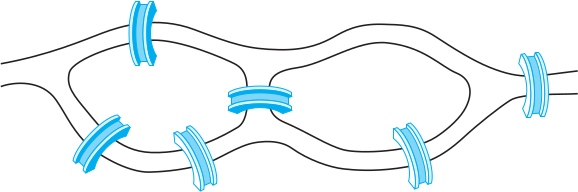
\includegraphics[width=0.5\textwidth]{not-konigsberg-graph}
\end{center}

\paragraph{Í bók:} Exercise 10.5.10

\question Fyrir hvaða gildi á $n$ hafa eftirfarandi net Euler-rás? En Hamilton-rás? Útskýrið.

\begin{enumerate}[a)]
 \item $K_n$
 \item $W_n$
\end{enumerate}

\paragraph{Í bók:} Hluti af Exercise 10.5.26 og Exercise 10.5.44

\section{Kafli 10.6}

\question Finnið léttasta veg á milli gefnu borganna í eftirfarandi neti:

\begin{center}
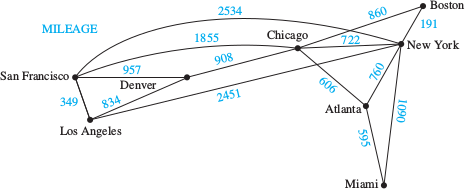
\includegraphics[width=0.6\textwidth]{graph-weighted-mileage}
\end{center}

\begin{enumerate}[a)]
 \item New York og Los Angeles
 \item Miami og Denver
\end{enumerate}

\paragraph{Í bók:} Hluti af Exercise 10.6.8

\question Sýnið að reiknirit Dijkstras finni ekki alltaf léttasta veg í neti sem inniheldur leggi með neikvæðri þyngd.

\paragraph{Ráðlegging:} Finnið dæmi um net með neikvæðri þyngd á legg sem reiknirit Dijkstras klikkar á og útskýrið hvað fer úrskeiðis. Netið getur verið mjög lítið.

\paragraph{Í bók:} Exercise 10.6.24

\end{questions}


\end{document}